% !TeX program = lualatex
% !LW recipe=Build Beamer with LuaLaTeX
\documentclass[aspectratio=43,10pt]{beamer}

\usetheme[compress]{Ilmenau}
\usefonttheme{professionalfonts}

\usepackage{fontspec}
\usepackage{graphicx}
\usepackage{booktabs}
\usepackage{amsmath}
\usepackage{xcolor}
\usepackage{array}
\usepackage{tabularx}
\usepackage{microtype}
\usepackage{tikz}
\usetikzlibrary{arrows.meta,positioning}
\usepackage{hcmut-ilmenau}

\setsansfont{Latin Modern Sans}
\setmainfont{Latin Modern Roman}

\graphicspath{{assets/}{figures/}}

\title[Vietnamese AVSR for Laptop Recording Transcription]{Vietnamese Audio-Visual Speech Recognition Using AV-HuBERT with Joint CTC/Attention Decoding for Laptop-Based Record Transcription}
\author[Hoang Long, Gia An, Tien Dat, Gia Khanh]{Ngo Hoang Long \and Nguyen Gia An \and Nguyen Tien Dat \and Vo Van Gia Khanh}
\institute[HCMUT -- ML IoT Lab]{Ho Chi Minh City University of Technology -- VNUHCM\\Machine Learning \& IoT Lab (ML IoT)}
\date{September 6, 2026}

\begin{document}

\begin{frame}
  \vspace{0.18cm}
  \begin{center}
    \begin{beamercolorbox}[wd=0.92\textwidth,sep=0.72em,center,rounded=true]{title}
      \usebeamerfont{title}
      Vietnamese Audio-Visual Speech Recognition\par
      Using AV-HuBERT with Joint\par
      CTC/Attention Decoding\par
      for Laptop-Based Record Transcription
    \end{beamercolorbox}

    \vspace{0.12cm}
    {\footnotesize\bfseries\color{ClassicBlue}
      Course: Python and Machine Learning 2026 \textcolor{HCMUTInk}{-- Final Project}\par}
    \vspace{0.14cm}
    {\small
      \begin{tabular}{@{}cc@{}}
        Ngo Hoang Long & Nguyen Gia An \\
        Nguyen Tien Dat & Vo Van Gia Khanh
      \end{tabular}\par}

    \vspace{0.20cm}
    \makebox[\textwidth][l]{%
      \hspace*{0.70cm}%
      \begin{minipage}{0.88\textwidth}
        \begin{columns}[T,onlytextwidth]
          \begin{column}{0.47\textwidth}
            \centering
            
\includegraphics[height=1.00cm,trim=260 100 95 50,clip]{hcmut-logo.png}\par
            \vspace{0.08cm}
            {\fontsize{5.8}{6.8}\selectfont\bfseries
              Ho Chi Minh City University of Technology -- VNUHCM\par}
          \end{column}
          \begin{column}{0.47\textwidth}
            \centering
            
\includegraphics[height=1.00cm]{ml-iot-logo.png}\par
            \vspace{0.08cm}
            {\fontsize{5.8}{6.8}\selectfont\bfseries
              Machine Learning \& IoT Lab (ML IoT)\par}
          \end{column}
        \end{columns}
      \end{minipage}%
    }
  \end{center}

  \vfill
  \begin{center}
    {\scriptsize\insertdate\par}
  \end{center}
  \vspace{0.18cm}
\end{frame}

\begin{frame}{Outline}
  \tableofcontents[hideallsubsections]
\end{frame}

\section[Background]{Background}
\classicsectiondivider{From multimodal pretraining to Vietnamese AVSR.}

\subsection{AV-HuBERT Pretraining Pipeline}

\begin{frame}{Overview}
  \centering
  \vspace{-0.12cm}
  \begin{tikzpicture}[
    x=1cm,
    y=1cm,
    flow/.style={draw=ClassicNavy,thick,rounded corners=2pt,fill=ClassicSoft,
      align=center,minimum height=0.62cm,font=\scriptsize,inner sep=3pt},
    encoder/.style={flow,fill=HCMUTLightBlue!14},
    fusion/.style={flow,fill=green!12!white},
    target/.style={flow,fill=orange!16!white},
    loss/.style={flow,draw=red!70!black,fill=red!7!white},
    arrow/.style={-{Latex[length=2.1mm,width=1.4mm]},line width=0.65pt,draw=gray!80!black}
  ]
    % Input timelines
    \node[inner sep=0pt] (visual) at (-3.0,0.55)
      {
\includegraphics[width=4.55cm,height=0.60cm,keepaspectratio]{masked-visual-red.png}};
    \node[font=\tiny,below=0.02cm of visual] {Visual: $v_{1:T}\xrightarrow{M_v}\widetilde v_{1:T}$};
    \node[inner sep=0pt] (audio) at (3.0,0.55)
      {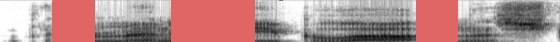
\includegraphics[width=4.55cm,height=0.60cm,keepaspectratio]{avhubert-audio-timesteps.png}};
    \node[font=\tiny,below=0.02cm of audio] {Audio: $a_{1:T}\xrightarrow{M_a}\widetilde a_{1:T}$};

    % Encoders and fused contextual representation
    \node[encoder,text width=3.25cm] (venc) at (-3.0,1.65)
      {\textbf{Visual encoder (ResNet-18)}\\[-0.05cm]$f_t^v=E_v(\widetilde v_t)$};
    \node[encoder,text width=3.25cm] (aenc) at (3.0,1.65)
      {\textbf{Audio encoder (Linear)}\\[-0.05cm]$f_t^a=E_a(\widetilde a_t)$};
    \node[fusion,text width=4.15cm] (fusion) at (0,2.85)
      {\textbf{Frame-wise fusion + modality dropout}\\[-0.05cm]
       $x_t=D_m\!\left([f_t^a;f_t^v]\right)$};
    \node[flow,text width=4.15cm,fill=ClassicBlue!11!white] (transformer) at (0,4.00)
      {\textbf{Transformer context encoder}\\[-0.05cm]
       $h_{1:T}=\operatorname{Transformer}(x_{1:T})$};
    \node[flow,text width=2.75cm] (prediction) at (-2.45,5.15)
      {\textbf{Cluster prediction}\\[-0.05cm]
       $p_t=\operatorname{Softmax}(Wh_t+b)$};

    % Pseudo-label branch
    \node[target,text width=1.85cm] (features) at (0.25,5.15)
      {MFCC / previous iteration\\[-0.05cm]$r_t^{(k-1)}$};
    \node[target,text width=1.35cm] (kmeans) at (2.55,5.15)
      {\textbf{K-means}};
    \node[target,text width=1.28cm] (targets) at (4.50,5.15)
      {Target IDs\\[-0.05cm]$z_t^{(k)}$};
    \node[loss,text width=4.35cm] (objective) at (0.85,6.30)
      {\textbf{Masked prediction objective}\\[-0.04cm]
       $\mathcal L_{\mathrm{pre}}=-\sum_{t\in M_a\cup M_v}\log p_t(z_t)$};

    % Main model path
    \draw[arrow] (visual.north) -- (venc.south);
    \draw[arrow] (audio.north) -- (aenc.south);
    \draw[arrow] (venc.north) -- (fusion.south west);
    \draw[arrow] (aenc.north) -- (fusion.south east);
    \draw[arrow] (fusion.north) -- (transformer.south);
    \draw[arrow] (transformer.north) -- (prediction.south);

    % Target and loss paths
    \draw[arrow] (features.east) -- (kmeans.west);
    \draw[arrow] (kmeans.east) -- (targets.west);
    \draw[arrow] (prediction.north) -- (objective.south west);
    \draw[arrow] (targets.north) -- (objective.south east);

  \end{tikzpicture}

  \note{[Sources] AV-HuBERT.pdf, Sections 3.2--3.4 and Equations 1--4; Weining Hsu, AAAI 2022 AV-HuBERT talk, slides 23--26. Visual structure is redrawn for this presentation. The visual and acoustic timeline strips were supplied by the user.}
\end{frame}


\subsection{AV-HuBERT Inference Pipeline}

\begin{frame}{Overview}
  \centering
  \vspace{-0.12cm}
  \begin{tikzpicture}[
    x=1cm,
    y=1cm,
    flow/.style={draw=ClassicNavy,thick,rounded corners=2pt,fill=ClassicSoft,
      align=center,minimum height=0.58cm,font=\scriptsize,inner sep=3pt},
    encoder/.style={flow,fill=HCMUTLightBlue!14},
    fusion/.style={flow,fill=green!12!white},
    decoder/.style={flow,fill=orange!16!white},
    search/.style={flow,draw=red!70!black,fill=red!7!white},
    output/.style={flow,fill=ClassicBlue!12!white},
    arrow/.style={-{Latex[length=2.1mm,width=1.4mm]},line width=0.65pt,draw=gray!80!black}
  ]
    % Synchronized inference inputs.
    \node[inner sep=0pt] (visual) at (-3.0,0.38)
      {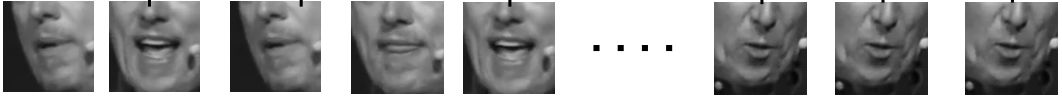
\includegraphics[width=4.35cm,height=0.56cm,keepaspectratio]{avhubert-visual-timesteps.png}};
    \node[font=\tiny,below=0.02cm of visual] {Visual sequence: $v_{1:T}$};
    \node[inner sep=0pt] (audio) at (3.0,0.38)
      {
\includegraphics[width=4.35cm,height=0.56cm,keepaspectratio]{avhubert-audio-timesteps_no_mask.png}};
    \node[font=\tiny,below=0.02cm of audio] {Audio sequence: $a_{1:T}$};

    % Shared AV-HuBERT encoder path.
    \node[encoder,text width=3.20cm] (venc) at (-3.0,1.40)
      {\textbf{Visual encoder (ResNet-18)}\\[-0.05cm]$f_t^v=E_v(v_t)$};
    \node[encoder,text width=3.20cm] (aenc) at (3.0,1.40)
      {\textbf{Audio encoder (Linear)}\\[-0.05cm]$f_t^a=E_a(a_t)$};
    \node[fusion,text width=4.35cm] (fusion) at (0,2.48)
      {\textbf{Frame-wise AV fusion}\\[-0.05cm]
       $x_t=[f_t^a;f_t^v]$\\[-0.04cm]
       {\tiny inference keeps both available streams}};
    \node[flow,text width=4.35cm,fill=ClassicBlue!11!white] (transformer) at (0,3.62)
      {\textbf{Transformer context encoder}\\[-0.05cm]
       $H=h_{1:T}=\operatorname{Transformer}(x_{1:T})$};

    % Two complementary decoding scores.
    \node[decoder,text width=3.30cm] (ctc) at (-1.90,4.78)
      {\textbf{CTC prefix scorer}\\[-0.05cm]
       $s_{\mathrm{CTC}}(y_{1:u}\mid H)$\\[-0.04cm]
       {\tiny monotonic alignment}};
    \node[decoder,text width=3.30cm] (attention) at (1.90,4.78)
      {\textbf{Attention decoder}\\[-0.05cm]
       $s_{\mathrm{Att}}(y_{1:u}\mid H)$\\[-0.04cm]
       {\tiny autoregressive context}};
    \node[search,text width=6.25cm] (beam) at (0,5.93)
      {\textbf{Joint beam search}\\[-0.04cm]
       $S(y_{1:u})=\lambda_{\mathrm{dec}}s_{\mathrm{CTC}}
       +(1-\lambda_{\mathrm{dec}})s_{\mathrm{Att}}$};
    \node[output,text width=4.55cm] (transcript) at (0,6.83)
      {\textbf{Vietnamese transcript}\quad
       $\widehat Y=\arg\max_Y S(Y)$};

    % Connectors follow the inference dataflow.
    \draw[arrow] (visual.north) -- (venc.south);
    \draw[arrow] (audio.north) -- (aenc.south);
    \draw[arrow] (venc.north) -- (fusion.south west);
    \draw[arrow] (aenc.north) -- (fusion.south east);
    \draw[arrow] (fusion.north) -- (transformer.south);
    \draw[arrow] (ctc.south |- transformer.north) -- (ctc.south);
    \draw[arrow] (attention.south |- transformer.north) -- (attention.south);
    \draw[arrow] (ctc.north) -- (ctc.north |- beam.south);
    \draw[arrow] (attention.north) -- (attention.north |- beam.south);
    \draw[arrow] (beam.north) -- (transcript.south);
  \end{tikzpicture}

  \note{[Sources] AV-HuBERT.pdf, Section 3.4; ViCocktail Automated Multi-Modal Data Collection for Vietnamese Audio-Visual Speech Recognition.pdf, Section 2.2 and Figure 3; current inference configuration. The diagram reuses the deck's AV-HuBERT encoder visual language and removes training-only masked prediction, pseudo-label generation, and modality dropout.}
\end{frame}


\subsection{Evaluation Metrics}

\begin{frame}{Evaluation Metrics}
  \small
  \begin{columns}[T,onlytextwidth]
    \begin{column}{0.48\textwidth}
      \begin{block}{Word Error Rate (WER)}
        \centering
        \[
          \mathrm{WER}=\frac{S_w+D_w+I_w}{N_w}
        \]
        \raggedright
        \scriptsize
        Measures the proportion of reference word tokens that must be substituted, deleted, or inserted.

        \vspace{0.08cm}
        \textbf{Reference:} hôm nay trời \textcolor{ClassicBlue}{đẹp}\\
        \textbf{Prediction:} hôm nay trời \textcolor{red!75!black}{lạnh}

        \vspace{0.05cm}
        $S_w=1,\ D_w=0,\ I_w=0,\ N_w=4$
        \[
          \mathrm{WER}=\frac{1}{4}=25\%
        \]
      \end{block}
    \end{column}
    \begin{column}{0.48\textwidth}
      \begin{block}{Character Error Rate (CER)}
        \centering
        \[
          \mathrm{CER}=\frac{S_c+D_c+I_c}{N_c}
        \]
        \raggedright
        \scriptsize
        Applies the same edit-distance calculation to characters, revealing smaller spelling and diacritic errors.

        \vspace{0.08cm}
        \textbf{Reference:} t\textcolor{ClassicBlue}{ô}i đang học\\
        \textbf{Prediction:} t\textcolor{red!75!black}{o}i đang học

        \vspace{0.05cm}
        $S_c=1,\ D_c=0,\ I_c=0,\ N_c=12$
        \[
          \mathrm{CER}=\frac{1}{12}\approx 8.3\%
        \]
      \end{block}
    \end{column}
  \end{columns}
  \note{[Sources] src/viavsr/evaluation/error_rates.py; src/viavsr/evaluation/text_normalization.py; tests/evaluation/test_error_rates.py. Spaces are included in the character sequence used by JiWER, so the normalized reference \textit{tôi đang học} contains 12 characters.}
\end{frame}

\subsection{ViCocktail}

\begin{frame}{ViCocktail}
  \small
  \begin{columns}[T,onlytextwidth]
    \begin{column}{0.48\textwidth}
      \begin{block}{Released resource}
        \begin{itemize}
          \item 271 hours, 195,240 utterances, and 2,411 speakers.
          \item Speaker-disjoint test set: 36 speakers, 1,167 utterances.
          \item Automated pipeline for shot detection, face tracking, active-speaker detection, AV sync, lip extraction, and ASR labeling.
          \item First public Vietnamese AVSR dataset with a strong AV-HuBERT baseline.
        \end{itemize}
      \end{block}
    \end{column}
    \begin{column}{0.48\textwidth}
      \begin{block}{What they showed}
        \centering
        \begin{tabular}{lcc}
          \toprule
          Model & Clean & Extreme \\
          \midrule
          Wave2Vec2 & 7.53\% & 70.01\% \\
          AV-HuBERT & 9.40\% & 18.39\% \\
          \bottomrule
        \end{tabular}
        \vspace{0.10cm}

        {\scriptsize Extreme: two interfering speakers at $-5$ dB SNR.}
      \end{block}
      \begin{alertblock}{What they DID NOT show}
        The paper evaluates acoustic interference, but does not directly study partial visual loss within an utterance, such as dropped or unavailable mouth frames.
      \end{alertblock}
    \end{column}
  \end{columns}
  \slidecitation{Source: Nguyen et al., \textit{ViCocktail}, Interspeech 2025, dataset overview and Table 2.}
  \note{[Sources] ViCocktail Automated Multi-Modal Data Collection for Vietnamese Audio-Visual Speech Recognition.pdf, Sections 2-5 and Table 2. The scope-gap statement is our interpretation of the documented construction and evaluation protocol.}
\end{frame}


\section[Questions]{Research Questions}
\classicsectiondivider{BIG QUESTION: Is the current Vietnamese baseline reliable enough to be deployed as a functional demo?}

\subsection{RQ1: Degradation}

\begin{frame}{RQ1: How Does Missing Video Affect Recognition Accuracy?}
  \small
  \begin{beamercolorbox}[wd=\textwidth,sep=0.70em,center,rounded=true]{block body}
    \textbf{Question:} How does recognition accuracy change as longer or more frequent visual gaps are introduced under laptop-recording conditions?
  \end{beamercolorbox}
  \vspace{0.16cm}

  \begin{columns}[T,onlytextwidth]
    \begin{column}{0.48\textwidth}
      \begin{block}{Evaluation setup}
        \begin{itemize}
          \item Keep the checkpoint, tokenizer, audio, and reference transcripts fixed.
          \item Apply paired deterministic interval masks at increasing visual-dropout ratios.
          \item Measure WER/CER relative to clean AV and repeat across multiple seeds.
        \end{itemize}
      \end{block}
    \end{column}
    \begin{column}{0.48\textwidth}
      \begin{block}{What we want to learn}
        \begin{itemize}
          \item Determine whether degradation is gradual or cliff-like.
          \item Is the released checkpoint already robust enough, or is fine-tuning needed?
        \end{itemize}
      \end{block}
    \end{column}
  \end{columns}
  \note{[Sources] configs and outputs for the paired full-test visual-dropout protocol. No numerical result is shown here; the Implementation section answers this question.}
\end{frame}

\subsection{RQ2: Strategy}

\begin{frame}{RQ2: How Should We Handle Missing Visual Frames?}
  \scriptsize
  Let $v_t$ be the visual input and $m_t\in\{0,1\}$ its availability ($1$: available, $0$: missing) at time step $t$.\\
  Write $\widetilde v_t=m_tv_t$, $f_t^a=E_a(a_t)$, and $f_t^v=E_v(\widetilde v_t)$, using the same encoders as in Background.
  \vspace{0.03cm}

  \renewcommand{\arraystretch}{1.20}
  \begin{tabularx}{\textwidth}{
    >{\bfseries\raggedright\arraybackslash}p{0.18\textwidth}
    >{\centering\arraybackslash}p{0.31\textwidth}
    >{\raggedright\arraybackslash}X}
    \toprule
    Strategy & Fused input $x_t$ & Runtime interpretation \\
    \midrule
    Corrupted AV &
    $[f_t^a;\,f_t^v]$ &
    Zero the missing frames and let the visual encoder process the corrupted sequence. \\
    Interval-gated AV &
    $[f_t^a;\,m_tf_t^v]$ &
    Zero the missing frames and suppress their visual features before fusion. \\
    Audio-only fallback &
    $[f_t^a;\,\mathbf{0}]\ \forall t$ &
    Discard the visual stream for the whole utterance and decode from audio only. \\
    \bottomrule
  \end{tabularx}
  \vspace{0.06cm}

  \begin{columns}[T,onlytextwidth]
    \begin{column}{0.48\textwidth}
      \begin{block}{Evaluation setup}
        Use the same utterance, audio, missing-frame mask, and dropout ratio for every strategy. Compare WER, CER, and inference time.
      \end{block}
    \end{column}
    \begin{column}{0.48\textwidth}
      \begin{alertblock}{What we want to learn}
        When visual input is unreliable, is it better to explicitly suppress visual features at missing time steps, or let the model infer from the corrupted input and the remaining audio-visual context?
      \end{alertblock}
    \end{column}
  \end{columns}
  \note{[Sources] AV-HuBERT.pdf, Section 3.3 and Equations 2-4; src/viavsr/inference/recognition.py. Interval gating is a project-side runtime intervention, not the original AV-HuBERT modality-dropout mechanism. No benchmark result is shown here. Notation follows Background: audio-first concatenation, v for visual input, and a tilde for modified input. Here the modification is runtime zeroing, not the pretraining replacement operation. The expression E_v(tilde v_t) is time-indexed shorthand: the visual frontend processes the sequence and can use neighboring frames, so a zero input frame need not yield a zero feature. The binary availability m_t is distinct from the sequence-level modality-dropout operator D_m.}
\end{frame}


\section[Implementation]{Implementation}
\classicsectiondivider{Answering the research questions with the released Vietnamese checkpoint and paired missing-visual tests.}

\subsection{RQ1 Result}

\begin{frame}{RQ1 Result: Accuracy Degrades Gradually}
  \small
  \centering
  \renewcommand{\arraystretch}{1.25}
  \begin{tabular}{lrr}
    \toprule
    Condition & Corpus WER & Change from clean \\
    \midrule
    Clean AV & 9.41\% & 0.00 \\
    AV, 10\% visual dropout & 9.44\% & +0.03 \\
    AV, 30\% visual dropout & 10.02\% & +0.61 \\
    AV, 50\% visual dropout & 11.05\% & +1.64 \\
    Audio-only (100\% visual dropout) & 13.64\% & +4.23 \\
    \bottomrule
  \end{tabular}
  \vspace{0.12cm}

  {\scriptsize Full ViCocktail test set. Audio is unchanged; only the visual stream is corrupted using deterministic interval masks.}
  \vspace{0.18cm}

  \vspace{0.25cm}
  \begin{minipage}{0.94\textwidth}
    \raggedright
    Across the tested dropout levels, \textbf{recognition degrades gradually}. At 50\% visual dropout, WER rises by 1.64 percentage points from clean AV, but remains 2.59 points below audio-only. These results suggest that \textbf{partial visual input remains useful} when audio is preserved.
  \end{minipage}
  \vspace{0.25cm}

  \note{[Sources] outputs/runpod_vicocktail_test_full_610f2a6/benchmark_report.json and results.jsonl. Dropout rows use corrupted AV; audio is unchanged and the same dropout masks are paired across modes.}
\end{frame}

\subsection{RQ2 Result}

\begin{frame}{RQ2 Result: Corrupted AV Performs Best}
  \small
  \centering
  \renewcommand{\arraystretch}{1.10}
  \begin{tabular}{lrrrr}
    \toprule
    Inference mode & 0\% & 10\% & 30\% & 50\% \\
    \midrule
    Clean AV & 9.41 & -- & -- & -- \\
    Corrupted AV & -- & \textbf{9.44} & \textbf{10.02} & \textbf{11.05} \\
    Interval-gated AV & -- & 9.59 & 10.29 & 11.11 \\
    Audio only & 13.64 & -- & -- & -- \\
    \bottomrule
  \end{tabular}
  \vspace{0.03cm}

  {\scriptsize Corpus WER (\%); identical dropout intervals and unchanged audio are used for paired comparison.}
  \vspace{0.08cm}

  \vspace{0.35cm}
  \begin{minipage}{0.94\textwidth}
    \raggedright
    The results support \textbf{preserving the remaining visual input} so the model can use its learned audio-visual representations and \textbf{temporal context within the utterance}. Under the tested visual gaps, Corrupted AV gives lower WER than explicitly zeroing visual features or discarding the visual stream entirely.
  \end{minipage}
  \vspace{0.25cm}

  \note{[Sources] outputs/runpod_vicocktail_test_full_610f2a6/benchmark_report.json and results.jsonl; src/viavsr/inference/recognition.py. Automatic routing is omitted because the comparison isolates the three underlying mechanisms directly. Temporal context refers to information across time steps within the same utterance, not surrounding sentences. The observed WER ranking supports this deployment choice but does not establish that masked pretraining caused the advantage or that the small differences over interval gating are statistically significant.}
\end{frame}

\subsection{Contributions}

\begin{frame}{Contribution and Future Work}
  \small
  \begin{columns}[T,onlytextwidth]
    \begin{column}{0.48\textwidth}
      \begin{block}{Contribution}
        \begin{itemize}
          \setlength{\itemsep}{0.12cm}
          \item Paired robustness evaluation on the ViCocktail test split across three missing-visual modes.
          \item A complete pipeline from raw recordings through mouth-ROI preprocessing to CTC/Attention decoding.
          \item A GPU-backed web demo exposing the mouth ROI, transcript, and runtime.
        \end{itemize}
      \end{block}
    \end{column}
    \begin{column}{0.48\textwidth}
      \begin{block}{Future work}
        \begin{itemize}
          \setlength{\itemsep}{0.12cm}
          \item Build a Vietnamese video-conferencing benchmark with paired local and received recordings from Zoom, Google Meet, and Microsoft Teams.
          \item Evaluate compression, frame loss, audio enhancement, and A/V desynchronization.
          \item Fine-tune the baseline and test generalization to unseen speakers and platforms.
        \end{itemize}
      \end{block}
    \end{column}
  \end{columns}
  \vspace{0.12cm}
  \note{Current contributions are evaluation and engineering using the released Vietnamese checkpoint, not a newly trained model. Proposed research is inspired by Huang et al., When AVSR Meets Video Conferencing: Dataset, Degradation, and the Hidden Mechanism Behind Performance Collapse, CVPR 2026, https://arxiv.org/abs/2603.22915. That work studies VC distribution shift, including speech enhancement and transmission effects. Zoom, Google Meet, and Microsoft Teams are the team's proposed platform coverage, not a claim about the paper's evaluated platforms. Collect consented Vietnamese speech with verified transcripts, pair the source and received recordings, document device/network/platform settings, keep source utterances and speakers disjoint across splits, and hold out platforms to test transfer. This benchmark would complement ViCocktail with VC-specific conditions; superiority has not been established. Dataset collection and fine-tuning remain future work.}
\end{frame}

\subsection{Reference}

\begin{frame}{Reference}
  \footnotesize
  \begin{list}{}{%
    \setlength{\leftmargin}{0.60cm}%
    \setlength{\labelwidth}{0.45cm}%
    \setlength{\labelsep}{0.15cm}%
    \setlength{\itemsep}{0.45cm}%
  }
    \item[{[1]}] B. Shi, W.-N. Hsu, K. Lakhotia, and A. Mohamed,
      \textit{Learning audio-visual speech representation by masked multimodal cluster prediction},
      in \textit{Proc. Int. Conf. Learn. Represent. (ICLR)}, 2022.

    \item[{[2]}] T.-B. Nguyen, T. V. Nguyen, Q. T. Do, and C. M. Luong,
      \textit{ViCocktail: Automated multi-modal data collection for Vietnamese audio-visual speech recognition},
      in \textit{Proc. Interspeech}, 2025, pp. 166--170,
      doi: \href{https://doi.org/10.21437/Interspeech.2025-1559}{10.21437/Interspeech.2025-1559}.

    \item[{[3]}] Y. Dai \textit{et al.},
      \textit{A study of dropout-induced modality bias on robustness to missing video frames for audio-visual speech recognition},
      in \textit{Proc. IEEE/CVF Conf. Comput. Vis. Pattern Recognit. (CVPR)},
      2024, pp. 27445--27455.
  \end{list}
  \note{Bibliographic metadata verified against the AV-HuBERT authors' ICLR 2022 record, ISCA Archive for ViCocktail, and the CVF CVPR 2024 proceedings record. The CVPR citation uses the published CVF author list and pagination rather than the differing arXiv metadata. Paper titles are clickable.}
\end{frame}

\begin{frame}[plain]
  \centering
  \vfill
  {\color{ClassicNavy}\bfseries\fontsize{27}{34}\selectfont
    THANK YOU\\[0.22cm]
    FOR LISTENING\par}
  \vfill
\end{frame}


\end{document}
